\documentclass[a4paper,12pt]{report}
\usepackage[utf8]{inputenc}
\usepackage{amsmath}
\usepackage{graphicx}
\usepackage{listings}
\usepackage{tikz}
\usepackage[T1]{fontenc}
\usepackage{color}
\usetikzlibrary{arrows,automata}
\definecolor{pythonred}{rgb}{0.6,0,0} % for strings
\definecolor{pythongreen}{rgb}{0.25,0.5,0.35} % comments
\definecolor{pythonpurple}{rgb}{0.5,0,0.35} % keywords
	\definecolor{pythondocblue}{rgb}{0.25,0.35,0.75} % javadoc
	 
	\lstset{language=python,
	basicstyle=\ttfamily,
	keywordstyle=\color{pythonpurple}\bfseries,
	stringstyle=\color{pythonred},
	commentstyle=\color{pythongreen},
	morecomment=[s][\color{pythondocblue}]{/**}{*/},
	numbers=left,
	numberstyle=\tiny\color{black},
        stepnumber=2,
	numbersep=10pt,
	tabsize=4,
	showspaces=false,
	showstringspaces=false}

% Title Page

 \title{\bfseries\huge \textcolor{purple}{\underline {EEP-703 Computer Network Lab}} \\{\textcolor{blue}{Assignment4-Client-Server Socket Programming using UDP}}}
\author{\bfseries\large\textcolor{black}  {Harshit  Kumar Gupta}\\ {\textcolor{black} {2013EET2369 }}\\

\includegraphics[width=3cm,height=3.4cm]{./iit.png}\\\noindent Computer Technology\\
\noindent Department Of Electrical Engineering\\IIT DELHI}
% iit.png: 282x282 pixel, 72dpi, 9.95x9.95 cm, bb=0 0 282 282
\begin{document}
\maketitle
\tableofcontents


\chapter{\textcolor{blue}{\underline {PROBLEM STATEMENT}}}
\noindent 
         Basics of Network Programming: An introduction to the basics of writing client-server stubs in JAVA in UNIX
environment.\\\\
\begin{enumerate}
 \item Problem Statement (a)
  Using Implement this: a client sends an AWK script to the server. The AWK script on execution
generates a message. Server will (first) execute the script and (then) send the output message
back to client. To avoid spamming, server will accept the AWK script only after authentication
with a secret-code. This secret-code is pre­known to all the true clients.
\item Problem Statement (b)
Extend the above scenario to serve multiple clients simultaneously. The server should be able to
keep track of up to 5 simultaneous users. However, server should accept the AWK script as a
file only from the first client who makes a request. Server should make the AWK file into an
executable, execute it locally and send the generated message back to the client.
\item Problem Statement (c)
Extend the above scenario so that the server broadcasts the output message to all the available
clients. Also provide the functionality to broadcast a custom message entered by ADMIN1. All the
clients (except the 1st one) should stay only in listen state.
\end{enumerate}

 



\begin{center}
\chapter{\textcolor{blue}{\underline {ABSTRACT}}}
\end{center}
\noindent The Intention of the JAVA Code is to make use of Socket Programming to create a Server and a Socket Client on a UDP approach
	  where we are supposed to send AWK script file from the Client side and send it to the Server.
	  The Server then in return send backs the entire record and displays it on the Client terminal.

\begin{center}
\chapter{\textcolor{blue}{\underline {INTRODUCTION}}}
\end{center}
\noindent  In all computer networks, one of the computers acts as a server (for applications, data, services)
to client computers. In this assignment, we will learn how to develop the JAVAcode which is
used to program this functionality on the client and on the server.\\\\
	  JAVA is one of the most widely used programming languages of all time, and JAVA compilers are available for the majority of available computer architectures and operating systems.
, 
UDP is a simple transport-layer protocol. The application writes a message to a UDP socket, which is then encapsulated in a UDP datagram, which is further encapsulated in an IP datagram, which is sent to the destination.

There is no guarantee that a UDP will reach the destination, that the order of the datagrams will be preserved across the network or that datagrams arrive only once.
The problem of UDP is its lack of reliability: if a datagram reaches its final destination but the checksum detects an error, or if the datagram is dropped in the network, it is not automatically retransmitted.

Each UDP datagram is characterized by a length. The length of a datagram is passed to the receiving application along with the data.
No connection is established between the client and the server and, for this reason, we say that UDP provides a connection-less service. 
	
\begin{center}
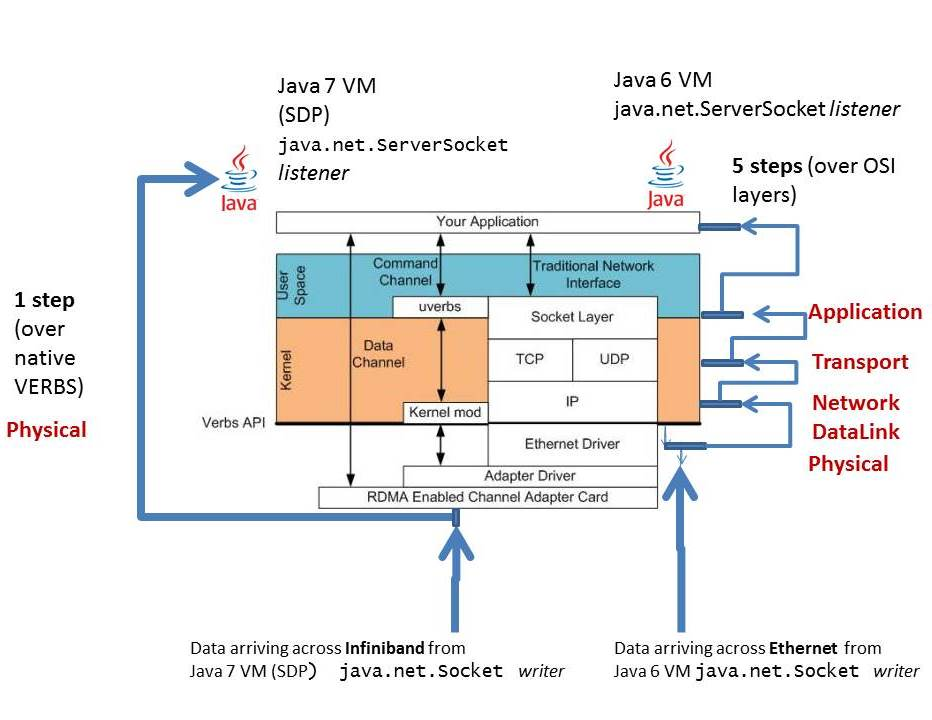
\includegraphics[width=12 cm,height=12 cm]{./flow.jpg}  
\end{center}
\begin{center}
\chapter{\textcolor{blue}{\underline {SPECIFICATIONS AND ASSUMPTIONS}}}
\end{center}
\section*{Specifications}
\begin{enumerate}
 

\item Client must provide authentication to send the awkscript to the server.
\item buffer size used is 1024 as it is sufficient.
\item The input file awkscript.awk is stored in the same path.
\item Socket Programming has been implemented in C language.
\end{enumerate}

\section*{Assumptions}
\begin{enumerate}
\item There are as such no multiple entries for the same client.

\item Error handling has been done accordingly for non existent records or as such.
\end{enumerate}
 
\begin{center}
\chapter{\textcolor{blue}{\underline {LOGIC USED/METHODOLOGY}}}
\end{center}
The methodology that is used for developing this project work is defined below:
\begin{enumerate} 
\item First of all a Server is To be Created and the port no is defined.
\item The Server Code also connects to the awkscript File.
\item A buffer is defined so as to save the Input file.
\item Now the Socket function is called and structure Intialised.

\item Now the input Search string say name is sent to the server.
\item Server executes awkscript and returns the corresponding Record value.
\item If the User enters some Invalid value , the error message is displayed.
\end{enumerate}

\begin{center}
\chapter{\textcolor{blue}{\underline {FLOWCHART}}}
\end{center}
\noindent Flowchart\\
\begin{center}
 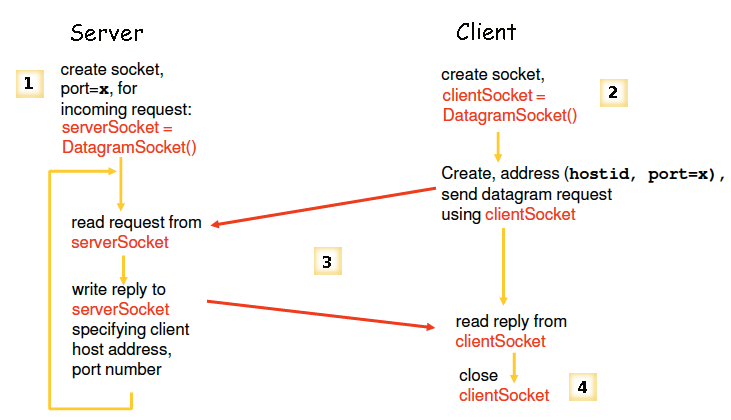
\includegraphics[width=12 cm,height=12 cm]{./client-server-udp.png}
 % UDP Flow.JPG: 576x270 pixel, 96dpi, 15.24x7.14 cm, bb=0 0 432 203
\end{center}


\begin{center}
\chapter{\textcolor{blue}{\underline {Execution Directives}}}
\end{center}
\noindent \\ In the terminal of LINUX system the following commands are executed in order to create a network topology and its analysis.\\
\begin{enumerate}
  \item Simply Compile the file writing java *.java
  \item Start server using java UDPServer
  
  \item Now Simply run client using java UDPClient
\item close -----close the comnnection
\item execawk awkfile inputfile -----execute awkfile and gives output
\item execawk awkfile inputfile -b -----execute awkfile and broadcasts output
\item wall message -----------broadcast message to all users
\item wall -f filename ------------- broadcast content of file
\end{enumerate}



\begin{center}
\chapter{\textcolor{blue}{\underline {RESULTS AND CONCLUSIONS}}}\end{center}
\noindent We find that for the given code seems to work perfectly fine and server accepts and executes the awkscript perfectly well.
\begin{center}
 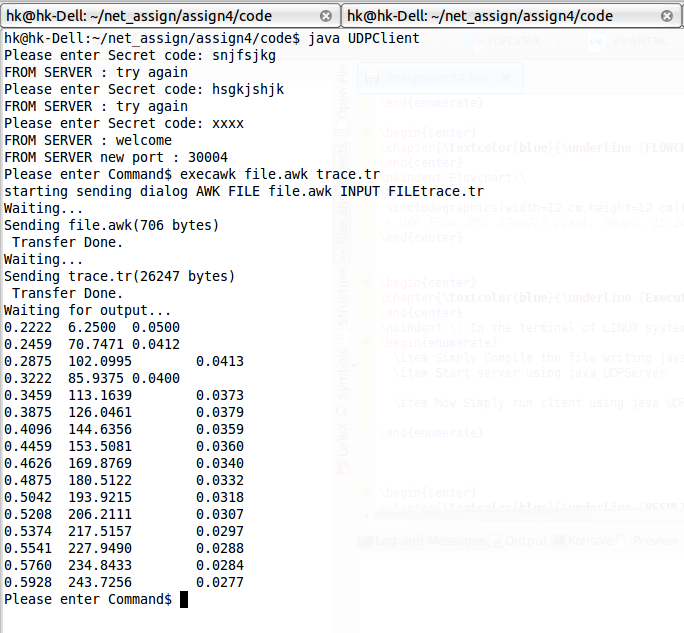
\includegraphics[width=12 cm,height=12 cm]{./Screenshot.png}
 % UDP Flow.JPG: 576x270 pixel, 96dpi, 15.24x7.14 cm, bb=0 0 432 203
\end{center}


\end{document}  